% Template per generare

\documentclass[a4paper,11pt]{article}
\usepackage{lmodern}
\renewcommand*\familydefault{\sfdefault}
\usepackage{sfmath}
\usepackage[utf8]{inputenc}
\usepackage[T1]{fontenc}
\usepackage[italian]{babel}
\usepackage{indentfirst}
\usepackage{graphicx}
\usepackage{tikz}
\newcommand*\circled[1]{\tikz[baseline=(char.base)]{
		\node[shape=circle,draw,inner sep=2pt] (char) {#1};}}
\usepackage{enumitem}
% \usepackage[group-separator={\,}]{siunitx}
\usepackage[left=2cm, right=2cm, bottom=3cm]{geometry}
\frenchspacing

\newcommand{\num}[1]{#1}

% Macro varie...
\newcommand{\file}[1]{\texttt{#1}}
\renewcommand{\arraystretch}{1.3}
\newcommand{\esempio}[2]{
\noindent\begin{minipage}{\textwidth}
\begin{tabular}{|p{11cm}|p{5cm}|}
	\hline
	\textbf{File \file{input.txt}} & \textbf{File \file{output.txt}}\\
	\hline
	\tt \small #1 &
	\tt \small #2 \\
	\hline
\end{tabular}
\end{minipage}
}

% Dati del task
\newcommand{\gara}{Olimpiadi Italiane di Informatica - Selezioni Territoriali 2013}
\newcommand{\nome}{Trova la parola}
\newcommand{\nomebreve}{trovaparola}

\begin{document}


% Intestazione
\noindent{\Large \gara}
\vspace{0.5cm}

\noindent{\Huge \textbf \nome~(\texttt{\nomebreve})}
\vspace{0.2cm}\\
\noindent{\large \textsc{Difficoltà D=2}}

% Descrizione del task
\section*{Descrizione del problema}

\begin{center}
  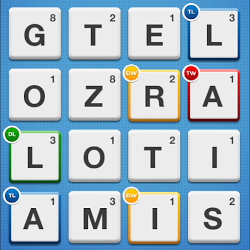
\includegraphics[width=5cm]{image00.png}
  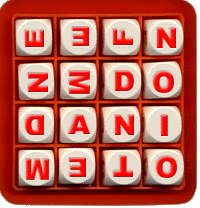
\includegraphics[width=5cm]{image02.png}
\end{center}

Visto il successo del gioco Ruzzle, che riprende il noto paroliere, i
giochi basati su trovare parole stanno vivendo un periodo molto
popolare.  Luciano, patito di giochi di tutti i tipi, ha ideato un
nuovo gioco, che funziona nel modo seguente: avete una griglia di
caratteri e una parola da trovare nella griglia, partendo dalla cella
in alto a sinistra.  Le uniche mosse consentite sono gli spostamenti a
destra o in basso. Ad esempio, considerate la seguente griglia e la
parola ``olimpiadi'':

\begin{table}[h]
  \centering
  \begin{tabular}{|c|c|c|c|c|c|c|}
    \hline
    O & L & I & V & E & N & T \\ \hline
    G & Q & M & P & W & E & R \\ \hline
    G & T & R & I & A & Y & E \\ \hline
    I & U & I & C & D & P & E \\ \hline
    A & F & C & O & I & G & H \\ \hline
    J & K & X & C & V & R & S \\ \hline
    R & O & M & I & T & A & A \\ \hline
    S & T & A & N & L & E & E \\ \hline
  \end{tabular}
\end{table}

In questo caso, la sequenza di spostamenti è \texttt{DDBDBDBB},
rappresentando gli spostamenti a destra con il carattere \texttt{D} e
quelli in basso con il carattere \texttt{B}.  Non esiste alcuna
soluzione, invece, se la parola da cercare è ``olimpionico''.  Il
vostro compito consiste nello scrivere un programma che, ricevute in
ingresso una parola (da cercare) e una griglia, restituisca la
sequenza di spostamenti, qualora esista una soluzione, oppure stampi
``ASSENTE''.  Se dovessero esistere molteplici sequenze di spostamenti
corrette, è sufficiente stamparne una qualunque.

\section*{Dati di input}
Il file \verb'input.txt' è composto da $2+R$ righe.  La prima riga
contiene due interi positivi $R$ e $C$: le dimensioni della griglia,
ovvero il numero di righe $R$ e il numero di colonne $C$.  La riga
successiva contiene $P$, una parola da cercare, rappresentata da una
stringa lunga almeno $2$ caratteri (alfabetici maiuscoli) e al massimo
$R+C-1$ caratteri.  Le rimanenti $R$ righe del file contengono le
righe della griglia, rappresentate da stringhe di $C$ caratteri
alfabetici maiuscoli.

\section*{Dati di output}
Il file \verb'output.txt' è composto da una sola riga contenente una
stringa di testo: la sequenza di spostamenti necessari per trovare la
parola nella griglia, se la parola è presente, oppure la stringa
``ASSENTE'' (senza le virgolette).

% Assunzioni
\section*{Assunzioni}
\begin{itemize}[nolistsep, noitemsep]
  \item $2 \le R, C \le 100$
\end{itemize}

% Esempi
\section*{Esempio di input/output}
\esempio{
8 7

OLIMPIADI

OLIVENT

GQMPWER

GTRIAYE

IUICDPE

AFCOIGH

JKXCVRS

ROMITAA

STANLEE
}{DDBDBDBB}

\esempio{
8 7

OLIMPIONICO

OLIVENT

GQMPWER

GTRIAYE

IUICDPE

AFCOIGH

JKXCVRS

ROMITAA

STANLEE
}{ASSENTE}

\section*{Nota}
Un programma che restituisce sempre lo stesso valore, indipendentemente dai dati in \texttt{input.txt}, non totalizza alcun punteggio.

\end{document}
